\documentclass{beamer}
\usetheme{default}
\begin{document}

\begin{frame}{Stochastic blockmodels}

Idea: 
\begin{itemize}
\item Each actor belongs to a latent class. 
\item Model block-wise interactions (mixing rates).
\end{itemize}

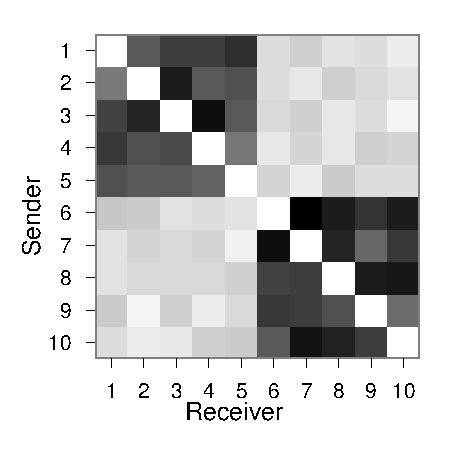
\includegraphics[scale=.5]{../../figs/synthetic/mat}
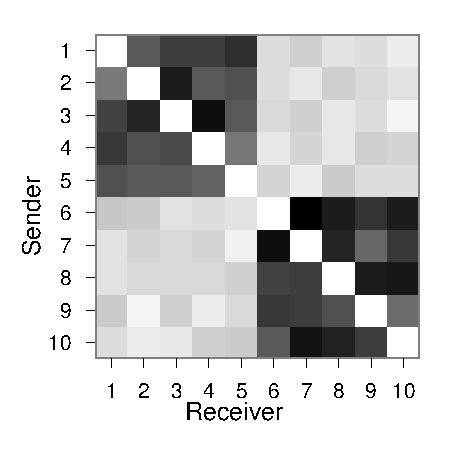
\includegraphics[scale=.5]{../../figs/synthetic/mat}
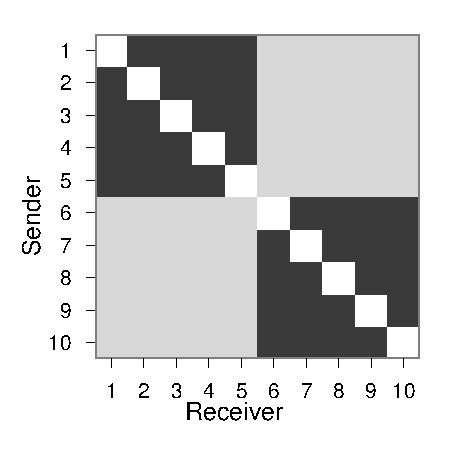
\includegraphics[scale=.5]{../../figs/synthetic/bm}

$$\boldsymbol{\eta} = \left[
\begin {array}{cc}
 \eta_{11}& \eta_{12} \\
 \eta_{11}& \eta_{12} 
\end {array}
\right]$$

% \begin{align*}
%$$ \eta = \left[ 
% \begin{tabular}{cc}
% \eta_{11}& \eta_{12} \\
% \eta_{11}& \eta_{12} 
% \end{tabular} 
%\right]$$
% \end{align*}

\begin{align*}
y_{ij} \sim& F(\eta_{z_i,z_j}) \\
z_i \sim& \mbox{Categorical}(\pi)
\end{align*}


\end{frame}

\end{document}
